\documentclass[a4paper,titlepage]{scrartcl}
\pagestyle{plain}
\usepackage[utf8]{inputenc}
\usepackage[T1]{fontenc}
\usepackage[german]{babel}
\usepackage{units}
\usepackage{floatrow}
\usepackage{amsmath,amssymb,amstext}
\usepackage{pgfplots,pgfplotstable}
\usepackage{numprint}
\usepackage{graphicx}

\newfloatcommand{capbtabbox}{table}[][\FBwidth]
\numberwithin{equation}{section}

\title{Auswertung vom Versuch P2-48: Ideales und reales Gas}
\author{Gruppe Di-22\\Jonas Müller, Genti Saliu}
\date{11. Mai 2014}

\begin{document}

\begin{titlepage}
\maketitle
\thispagestyle{empty}
\end{titlepage}

\newpage
\pagenumbering{roman}
\tableofcontents

\newpage
\pagenumbering{arabic}

\section{Spannungskoeffizient $\alpha$ von Luft und absoluter Nullpunkt}
In diesem Versuch sollten der Spannungskoeffizient $\alpha$ von Luft und der absolute Nullpunkt experimentell bestimmt werden.\\ \\
Wir sind dabei folgendermaßen vorgegangen: Zuerst wurden der Außendruck und die Raumtemperatur gemessen, es ergaben sich $t_R=\unit[21.4]{^{\circ}C}$ bzw. $p=\unit[746.3]{torr}$.\\
Dann legten wir den Nullpunkt im festen Schenkel des Gasthermometers fest. Wir lasen die Höhendifferenz vom Quecksilber im Manometer beim Raumtemperatur ab, dann kühlten wir den Rezipienten in einem Eisbad auf $\unit[1]{^{\circ} C}$ ab. Den bewegten Schenkel passten wir so an, dass die Quecksilbersäule im festen Schenkel wieder auf der Nullmarke stand. Unseren Erwartungen nach, entstand im Glaskolben aufgrund der Abkühlung Unterdruck, deshalb ist die Quecksilbersäule im Schenkel nach oben gestiegen. Anschließend erfolgte das Ablesen der Höhendifferenz der Quecksilbersäulen.\\
Danach haben wir den Glaskolben in einem Dampfbad bis zur Siedestemperatur des Wassers gebracht und sind analog wie oben vorgegangen. Im Gegensatz dazu entstand aufgrund der Erwärmung Überdruck und die Quecksilbersäule sank im festen Schenkel unter die Nullmarke.\\ \\
Da es sich um ein Quecksilbermessgerät handelt, verwenden wir für die Druckangabe durchgehend die Einheit \emph{torr}. Ein Millimeter Höhenunterschied entspricht dabei einem Druckunterschied von $\unit[1]{torr}$.\\ \\
Den Gesamtdruck errechnet man aus der Summe von Aussendruck und Druckdifferenz:
\begin{equation*}
p_{ges}=p + \Delta p
\end{equation*}

\begin{table}[H]
\begin{tabular}{c|c|c}
	Temperatur $t [^{\circ} C]$ & Höhendifferenz $\Delta h [mm]$ & Gesamtdruck $p_{ges} [torr]$ \\
	\hline
	21.4 & 23 & 769.3 \\
	1 & 35 & 781.3 \\
	97.8 & 214 & 987.3 \\
\end{tabular}
\caption{Messungen am Jollyschen Gasthermometer}
\label{tab:aufgabe1}
\end{table}

Anzumerken sei, dass der Wert der Siedetemperatur, den wir mit einem Digitalthermometer gemessen haben, vom theoretischen Wert der Siedestemperatur abweicht. Letztere errechnet sich aus \cite{auswertung1}:
\begin{eqnarray*}
t_{sied}&=&100 + 0.03687 \cdot (p - 760) - 0.000022 \cdot (p-760)^2 \quad \text{wobei} \quad p = \unit[995]{hPa}\\
&=&\unit[107.45]{^{\circ} C}
\end{eqnarray*}
Dies entspricht einer Abweichung von $\unit[0.09]{\%}$.\\ \\
Jetzt können wir den Spannungskoeffizienten $\alpha$ der Luft bestimmen. Wir errechnen zwei Werte für den Koeffizienten, einmal mit und einmal ohne Berücksichtigung der thermischen Ausdehnung von Glas.

\begin{description}
\item[Ohne Berücksichtigung der thermischen Ausdehnung]
\begin{equation*}
\alpha_1=\frac{p_D - p_E}{p_E \cdot T_{sied}}
\end{equation*}
\item[Mit Berücksichtigung der thermischen Ausdehnung]
\begin{equation*}
\alpha = \alpha_1 + \frac{p_D}{p_E} \cdot \gamma \quad \text{, wobei $ \gamma=\unit[2.5 \cdot 10^{-5}]{\frac{1}{K}} $ der kubische Ausdehungskoeffizient ist }
\end{equation*}
\end{description}

Ausgehend von den gemessenen Werten:
\begin{itemize}
\item $p_E = \unit[781.3]{torr}=\unit[104164.77]{Pa}$
\item $p_D = \unit[987.3]{torr}=\unit[131629.17]{Pa}$
\item $t_{sied} = \unit[97.8]{^{\circ} C}$ bzw. $T_{sied} = \unit[370.8]{K}$
\end{itemize}
erhielten wir:
\begin{equation*}
\alpha_1=\unit[7.1100 \cdot 10^{-4}]{\frac{1}{K}} \quad \quad \alpha=\unit[7.1123 \cdot 10^{-4}]{\frac{1}{K}}
\end{equation*}
Die Abweichung des unkorrigierten vom korrigierten Spannungskoeffizienten beträgt $\unit[0.03]{\%}$.\\ \\
Der absolute Nullpunkt errechnet sich aus:
\begin{equation*}
T_0= - \frac{1}{\alpha}=\frac{1}{\unit[7.1123 \cdot 10^{-4}]{\frac{1}{K}}}= - \unit[1406]{K}
\end{equation*}

Leider passen unsere Ergebnisse überhaupt nicht mit den Literaturwerten überein. Auch nach mehrmaligem nach Rechnen konnten wir keinen mathematischen Fehler erkennen. Daher liegt der Fehler wohl bei einer ungenauen Messung, da auch der Stand der Quecksilbersäule nur schlecht abzulesen war.

\newpage

\section{Bestimmung des Adiabatenindex}
\subsection{Clement-Desormes-Methode}
Der Versuch besteht der Vorbereitung entsprechend aus 4 Schritten.  Wir sind folgendermaßen vorgegangen:
\begin{enumerate}
\item Dreiweghahn so gestellt, dass nur Glasbehälter und Pumpe verbunden waren.
\item Mit Pumpe Überdruck erzeugt und Glasbehälter und Manometer über Dreiweghahn verbunden.
\item Höhendifferenz abgelesen.
\item Über Ventil am Glasbehälter Höhenausgleich bzw. Druckausgleich vorgenommen (Ventil nur kurz geöffnet, um Wärmeaustausch zu vermeiden).
\item Gewartet bis sich Gleichgewicht einstellt und Höhendifferenz abgelesen.
\item 1-5 wurden 3 mal wiederholt.
\end{enumerate}

Durch dieses Vorgehen erhalten wir zwei Höhendifferenzen: $\Delta h_1$ die Höhendifferenz, die durch den mit der Pumpe erzeugten Überdruck im Schritt 1 und $\Delta h_2$ die Höhendifferenz, die durch die Druckdifferenz nach Einstellen des thermischen Gleichgewichts im Schritt 5, enstanden ist.

Wie in der Vorbereitungshilfe hergeleitet, berechnet man $\kappa$ durch:
\begin{equation*}
\kappa = \frac{\Delta p_1}{\Delta p_1 - \Delta p_2}
\end{equation*}
Da wir in diesem Versuch Öl anstatt Quecksilber verwenden, kann man die praktische Umrechnung von Höhendifferenz in Druck nicht vornehmen, es gilt aber:
\begin{equation*}
\Delta p=\Delta h \cdot \rho_{Oel} \cdot g
\end{equation*}
Einsetzen in $\kappa$ ergibt:
\begin{equation*}
\kappa=\frac{\Delta h_1}{\Delta h_1 - \Delta h_2}
\end{equation*}
Jetzt können wir $\kappa$ ausrechnen und erhalten aus den Messwerten folgende Tabelle:
\begin{table}[H]
\begin{tabular}{c|c|c}
	Höhendifferenz $\Delta h_1 [mm]$ & Höhendifferenz $\Delta h_2 [mm]$ & $\kappa$ \\
	\hline
	56 & 15 & 1.37 \\
	65 & 15 & 1.30 \\
	60 & 15 & 1.33 \\
\end{tabular}
\caption{Messungen nach der Clement-Desormes-Methode}
\label{tab:aufgabe21}
\end{table}

Es ergibt sich ein Mittelwert von $\kappa=1.33$. Das ist eine Abweichung von $\unit[5]{\%}$ gegenüber dem Literaturwert.

\subsection{Vergleichsmessung}
Wir haben der Versuch wiederholt und dabei im 4. Schritt beim Druckausgleich das Ventil länger offen gehalten haben. Wie zu erwarten, konnten wir im Schritt 5 nur eine sehr geringe Höhendifferenz messen:
\begin{table}[H]
\begin{tabular}{c|c|c}
	Höhendifferenz $\Delta h_1 [mm]$ & Höhendifferenz $\Delta h_2 [mm]$ & $\kappa$ \\
	\hline
	52 & 5 & 1.11 \\
\end{tabular}
\caption{Vergleichsmessung}
\label{tab:aufgabe22}
\end{table}
Man kann deutlich erkennen, dass es sich hier nicht um eine adiabatsche Zustandsänderung handeln kann, da der Wert für $\kappa$ stark vom Literaturwert abweicht ($\unit[20.7]{\%}$).

\section{Bestimmen von $\kappa$ mit der Schwingmethode}
Wir haben uns für die Methode von Rüchard entschieden.
\subsection{Methode von Rüchard}
Der Aufbau wurde bereits in der Vorbereitung erklärt. Es mussten vor und während der Durchführung einige Punkte beachtet werden:
\begin{itemize}
\item Glasrohr musste sauber sein
\item Stopfen mussten dicht sein
\item Glasrohr musste möglichst senkreicht sein
\item Die Kugel musste sauber sein
\end{itemize}
Die Geräte, die wir im Labor vorgefunden haben, erfüllten die ersten drei obigen Bedingungen. Die Erfüllung der vierten Bedingung stellten wir sicher, indem wir die Metallkugel nicht mit bloßer Hand angefasst haben.\\ \\
Wir haben die Kugel in das Glasrohr fallenlassen. Dabei hat sie angefangen zu schwingen und wir haben die Zeit gestoppt und die Anzahl der in dieser Zeit erfolgten Schwingungen gezählt. Ab ca. 10 Schwingungen wurde die Oszillation der Kugel so gering, dass man keine weitere Schwingung zuverlässig erkennen konnte.\\ \\
Direkt aus der Periodendauer erhält man laut Vorbereitung das gesuchte Verhältnis der spezifischen Wärmen:
\begin{equation*}
\kappa = \left( \frac{2 \pi}{T} \right)^2 \frac{m}{A^2} \cdot \frac{V_0}{p_0}
\end{equation*}
mit 
\begin{itemize}
\item $p_0=\unit[995]{hPa}=\unit[99500]{Pa}$
\item $V_0=\unit[10.58]{l}=\unit[0.01058]{m^3}$
\item $m=\unit[16.68]{g}=\unit[16.68 \cdot 10^{-3}]{kg}$
\item $A=\frac{\pi \cdot d^2}{4}=\frac{\pi \cdot (\unit[16]{mm})^2}{4}=\unit[2 \cdot 10^{-4}]{m^2}$
\end{itemize}
Die Messungen und die entsprechende $\kappa$ sind in Tabelle \ref{tab:aufgabe3} zusammengefasst:
\begin{table}[H]
\begin{tabular}{c|c|c|c}
	Schwingungsanzahl $n$ & Dauer $t [s]$ & Periodendauer $T [s]$ & $\kappa$ \\
	\hline
	8 & 9.08 & 1.14 & 1.35 \\
	5 & 5.73 & 1.15 & 1.32 \\
	8 & 8.10 & 1.01 & 1.72 \\
	8 & 8.91 & 1.11 & 1.42 \\
	6 & 6.78 & 1.13 & 1.37 \\
	8 & 8.96 & 1.12 & 1.40 \\
\end{tabular}
\caption{Messungen der Periodendauer der schwingenden Kugel}
\label{tab:aufgabe3}
\end{table}
Es ergibt sich ein Mittelwert von $\kappa=1.43$ (Abweichung vom Literaturwert $\unit[2.1]{\%}$). Der Median beträgt $\kappa=1.385$ (Abweichung vom Literaturwert $\unit[1]{\%}$). Es wäre sinnvoller den Median zu betrachten, da wir in unseren Messungen einen Ausreißer (1.72) haben und die Abweichung vom Literaturwert kleiner ist.
\section{Dampfdruckkurve einer Flüssigkeit}
In diesem Versuch stellen wir die Dampfdruckkurve (Abhängigkeit des Drucks von der Temperatur) von n-Hexan auf, wobei anzumerken ist, dass hier die Druckdifferenz aufgetragen wurde (Abbildung \ref{fig:aufgabe4}). Diese erhält man, wie in Aufgabe 1, aus der Höhendifferenz der Quecksilbersäulen. Dabei entspricht $\unit[1]{mm}$ Höhendifferenz einer Druckdifferenz $\unit[1]{torr}$.
\begin{figure}[H]
	\centering
	\begin{tabular}{@{}r@{}}
		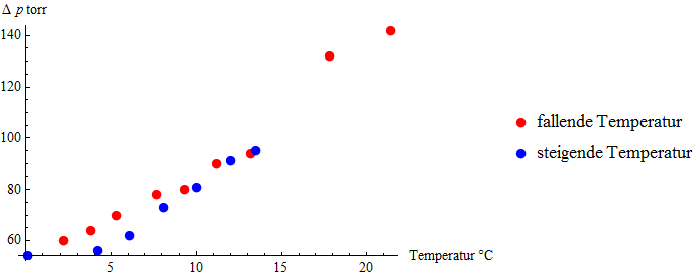
\includegraphics[width=1\textwidth]{bilder/aufgabe4.png}\\
	\end{tabular}
	\caption{Dampfdruckkurve von n-Hexan}
	\label{fig:aufgabe4}
\end{figure}
Tabelle \ref{tab:aufgabe4} zeigt die Ergebnisse unserer Messungen zu diesem Versuch.
\begin{table}[H]
\begin{tabular}{c|c|c|c}
	Temperatur T in $^{\circ C}$ & Höhe links $h_l [mm]$ & Höhe rechts $h_r [mm]$ & Druckdifferenz $\Delta p [torr]$ \\
	\hline
	21.4 & 466 & 324 & 142 \\
	17.8 & 461 & 329 & 132\\
	13.2 & 442 & 348 & 94 \\
	11.2 & 440 & 350 & 90 \\
	9.3 & 435 & 355 & 80 \\
	7.7 & 435 & 357 & 78 \\
	5.3 & 431 & 361 & 70 \\
	3.8 & 428 & 364 & 64 \\
	2.2 & 426 & 366 & 60 \\
	0.1 & 423 & 369 & 54 \\
	4.2 & 424 & 368 & 56 \\
	6.1 & 427 & 365 & 62 \\
	8.1 & 435 & 362 & 73 \\
	10.0 & 439 & 358 & 81 \\
	12.0 & 444 & 353 & 91 \\
	13.5 & 446 & 351 & 95 \\
\end{tabular}
\caption{Messergebnisse zur Dampfdruckkurve}
\label{tab:aufgabe4}
\end{table}
Entsprechend dem Aufbau aus der Vorbereitung haben wir n-Hexan über ein Wasserbad vom Raumtemperatur in $\approx \unit[2]{^{\circ} C}$-Schritten bis auf $\unit[0]{^{\circ} C}$ abgekühlt. Wir notierten bei jedem Schritt die Stände der Quecksilbersäulen im linken und rechten Schenkel des Manometers. Aus Zeitgründen wurden die Stände im linken Schenkel nur am Anfang und Ende gemessen und in der Auswertung die restlichen Werte ergänzt.\\
Anschließend wurde das Wasserbad mit kochendem Wasser wieder bis zur Raumtemperatur erwärmt. Da wir nicht genügend warmes Wasser zur Verfügung hatten, konnten wir die Flüssigkeit nur bis $\unit[13.5]{^{\circ C}}$ erwärmen.\\ \\
Um die Verdampfungsenthalpie machen wir uns der Beziehung aus der Vorbereitung zunutze:
\begin{equation*}
\ln{\frac{p}{p_0}}=-\frac{H_v}{T \cdot R}
\end{equation*}
Wir tragen $\ln{\frac{p}{p_0}}$ gegen $-\frac{1}{T \cdot R}$ in ein Diagramm auf, bestimmen wir die Ausgleichsgerade und erhalten deren Steiung als Verdampfungsenthalpie $H_v$. Dabei kann $p_0$ beliebig gewählt werden, da es die Steigung nicht verändert, nur die Verschiebung der Gerade entlang der y-Achse. Daher, aus $p=p_0+\Delta p$ und gewähltem $p_0=\unit[1]{torr}$ folgt:
\begin{equation}
\ln{\Delta p}=-\frac{H_v}{T \cdot R}
\end{equation} 
Wir haben unsere Messwerte in Mathematica eingegeben und lineare Regression über diese Daten durchgeführt. Die Gleichung der Regressionsgerade lautet:
\begin{equation*}
y=31476x + 17.8
\end{equation*}
Damit beträgt die gesuchte Verdamungsenthalpie $H_v=\unit[31476]{\frac{J}{mol}}$. Gegenüber dem Literaturwert von $H_v=\unit[28850]{\frac{J}{mol}}$ weist unser Ergebnis eine Abweichung von $\unit[9.1]{\%}$.\\
Die Ausgleichsgerade findet man in Abbildung \ref{fig:aufgabe41}.
\begin{figure}[H]
	\centering
	\begin{tabular}{@{}r@{}}
		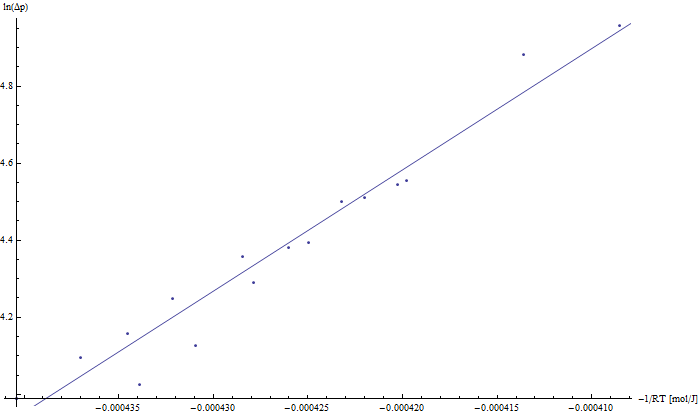
\includegraphics[width=0.8\textwidth]{bilder/aufgabe41.png}\\
	\end{tabular}
	\caption{Ausgleichsgerade zur Bestimmung von Verdampfungsenthalpie}
	\label{fig:aufgabe41}
\end{figure}

\bibliographystyle{plain}
\bibliography{quellen_auswertung}

\end{document}